\section{Previous work}
TODO

\subsection{Proxy-Based Cluster Architecture (2002)}
TODO
% The architecture proposed in this work takes its decisions based on dealing with the following issues (technological limitations at the time has to be taken in consideration): devices heterogeneity, low bandwidth, high latency, extended periods of disconnection, device power consumption and software interoperability.

\subsubsection{Architecture}
\begin{figure}[H]
    \centering
    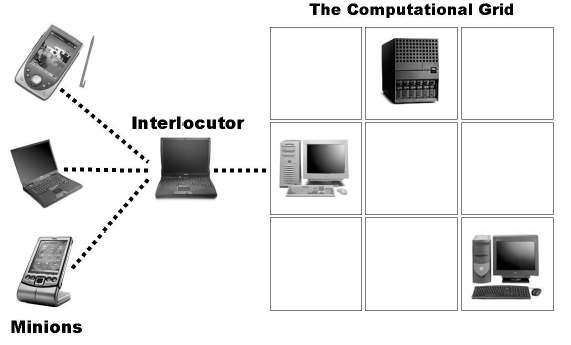
\includegraphics[scale=0.8]{document/chapters/chapter_3/images/2002_architecture.png}
    \caption{Proxy-Based Cluster Architecture \cite{integrating_mobile_devices_into_grid}}
    \label{fig:2002_architecture}
\end{figure}
This architecture revolves around the idea of having a \textbf{cluster} constituted by a number of \textbf{BASELINE} (Barely Adequate Systems Leveraging Internet NEtworking) \textbf{devices} that act as \textbf{\textit{Minions}}. Such BASELINE devices coexist (in the \textbf{same wireless network}) with a \textbf{proxy device} powerful enough to coordinate them. In this architecture, this proxy device is known as \textbf{\textit{Interlocutor}}; this machine runs a software that acts as a middleware with an existing Grid system.

\begin{quotation}
    \textit{"When a resource request arrives at the Interlocutor from a resource consumer, the request is handled by the Interlocutor. For simplicity, we proceed in this example with the assumption that the request is for CPU time to process incoming data. The interlocutor must decompose the request accordingly among its minions; [...]. After the problem has been distributed to the minions, the interlocutor waits for results and sends them back to the requester. The Interlocutor has the option of aggregating the data before responding with the result in order to amortize the cost of per-message communication overhead." \cite{integrating_mobile_devices_into_grid}}
\end{quotation}

\subsubsection{Interesting concepts and ideas}
One of the strengths of such architecture is \textbf{delegation}; Minions rely entirely on the Interlocutor, taking only the active decision (based on the user's will) to either participate or not to the Grid. Having such division in responsibilities \textbf{simplifies the software running on BASELINE devices} (which was the one mostly affected by compatibility issues given the number of OSes for PDAs) while moving such complexity on the stabler and more standardized Interlocutor.
Another advantage gained from this architecture is the \textbf{reduction of latency}. Since the devices operate under the same wireless network, a requestor that is located anywhere on the planet has only to execute a long request to the Interlocutor, while coordination in the cluster is almost instantaneous given the short distances.
The local coordination allows \textbf{managing resources more easily} since the responsibility of determinate whether certain resources are available and/or adequate becomes distributed between all Interlocutors.
\textbf{Device discovery is also greatly simplified} since the Grid services do not actually need to discover every single BASELINE device but only Interlocutors.
Furthermore, \textbf{the Interlocutor hides devices heterogeneity from the Grid}, allowing also to possibility to apply mechanisms to compensate for BASELINE devices performances.

While using a local Interlocutor seems very effective, every benefit gained by the use of it comes at the cost of a great limitation: \textbf{when it comes to practically scaling the Grid, having the devices operating under the same local network makes extremely more difficult for volunteers to offer their devices}. It is still possible to use some sort of variation of an Interlocutor, but this obviously comes at the cost of loosing some benefits such the reduction of latency while operating in the same network.

\subsection{Mobile-to-Grid Middleware (2005)}
TODO

\subsubsection{Architecture}
TODO

\subsubsection{Protocols}
TODO

\subsubsection{Interesting concepts and ideas}
TODO

\subsection{Autonomous Mobile Middleware (2006)}
TODO

\subsubsection{Architecture}
TODO

\subsubsection{Protocols}
TODO

\subsubsection{API examples}
TODO

\subsubsection{Interesting concepts and ideas}
TODO